% BioNetFlux Typical Experiment Workflow Diagram
% To be included in documentation

\documentclass{standalone}
\usepackage{tikz}
\usepackage{xcolor}
\usepackage{fontspec}
\usetikzlibrary{shapes,arrows,positioning,fit,backgrounds,calc}

% Define colors matching documentation theme
\definecolor{configcolor}{RGB}{255, 165, 0}    % Orange for configuration
\definecolor{geometrycolor}{RGB}{0, 128, 128}  % Teal for geometry
\definecolor{problemcolor}{RGB}{70, 130, 180}  % Steel blue for problems
\definecolor{solvercolor}{RGB}{220, 20, 60}    % Crimson for solvers
\definecolor{outputcolor}{RGB}{34, 139, 34}    % Forest green for output

% Define styles
\tikzset{
    % Box styles
    configbox/.style={rectangle, rounded corners, minimum width=2.5cm, minimum height=1cm, 
                     align=center, draw=configcolor, fill=configcolor!20, thick},
    geometrybox/.style={rectangle, rounded corners, minimum width=2.5cm, minimum height=1cm,
                      align=center, draw=geometrycolor, fill=geometrycolor!20, thick},
    problembox/.style={rectangle, rounded corners, minimum width=2.5cm, minimum height=1cm,
                      align=center, draw=problemcolor, fill=problemcolor!20, thick},
    solverbox/.style={rectangle, rounded corners, minimum width=2.5cm, minimum height=1cm,
                     align=center, draw=solvercolor, fill=solvercolor!20, thick},
    outputbox/.style={rectangle, rounded corners, minimum width=2.5cm, minimum height=1cm,
                     align=center, draw=outputcolor, fill=outputcolor!20, thick},  
    % Decision diamond
    decision/.style={diamond, minimum width=1.5cm, minimum height=1cm,
                    text centered, draw=black, fill=yellow!30, thick},         
    % Process styles
    process/.style={rectangle, minimum width=2cm, minimum height=0.8cm,
                   text centered, draw=black, fill=white, thick},   
    % Arrow styles
    arrow/.style={->, >=stealth, thick},
    configarrow/.style={->, >=stealth, thick, configcolor},
    geometryarrow/.style={->, >=stealth, thick, geometrycolor},
    problemarrow/.style={->, >=stealth, thick, problemcolor},
    solverarrow/.style={->, >=stealth, thick, solvercolor},
    outputarrow/.style={->, >=stealth, thick, outputcolor},  
    % Text styles
    methodtext/.style={font=\scriptsize\ttfamily, align=center, text=teal},
    classtext/.style={font=\small\bfseries}
}

\begin{document}
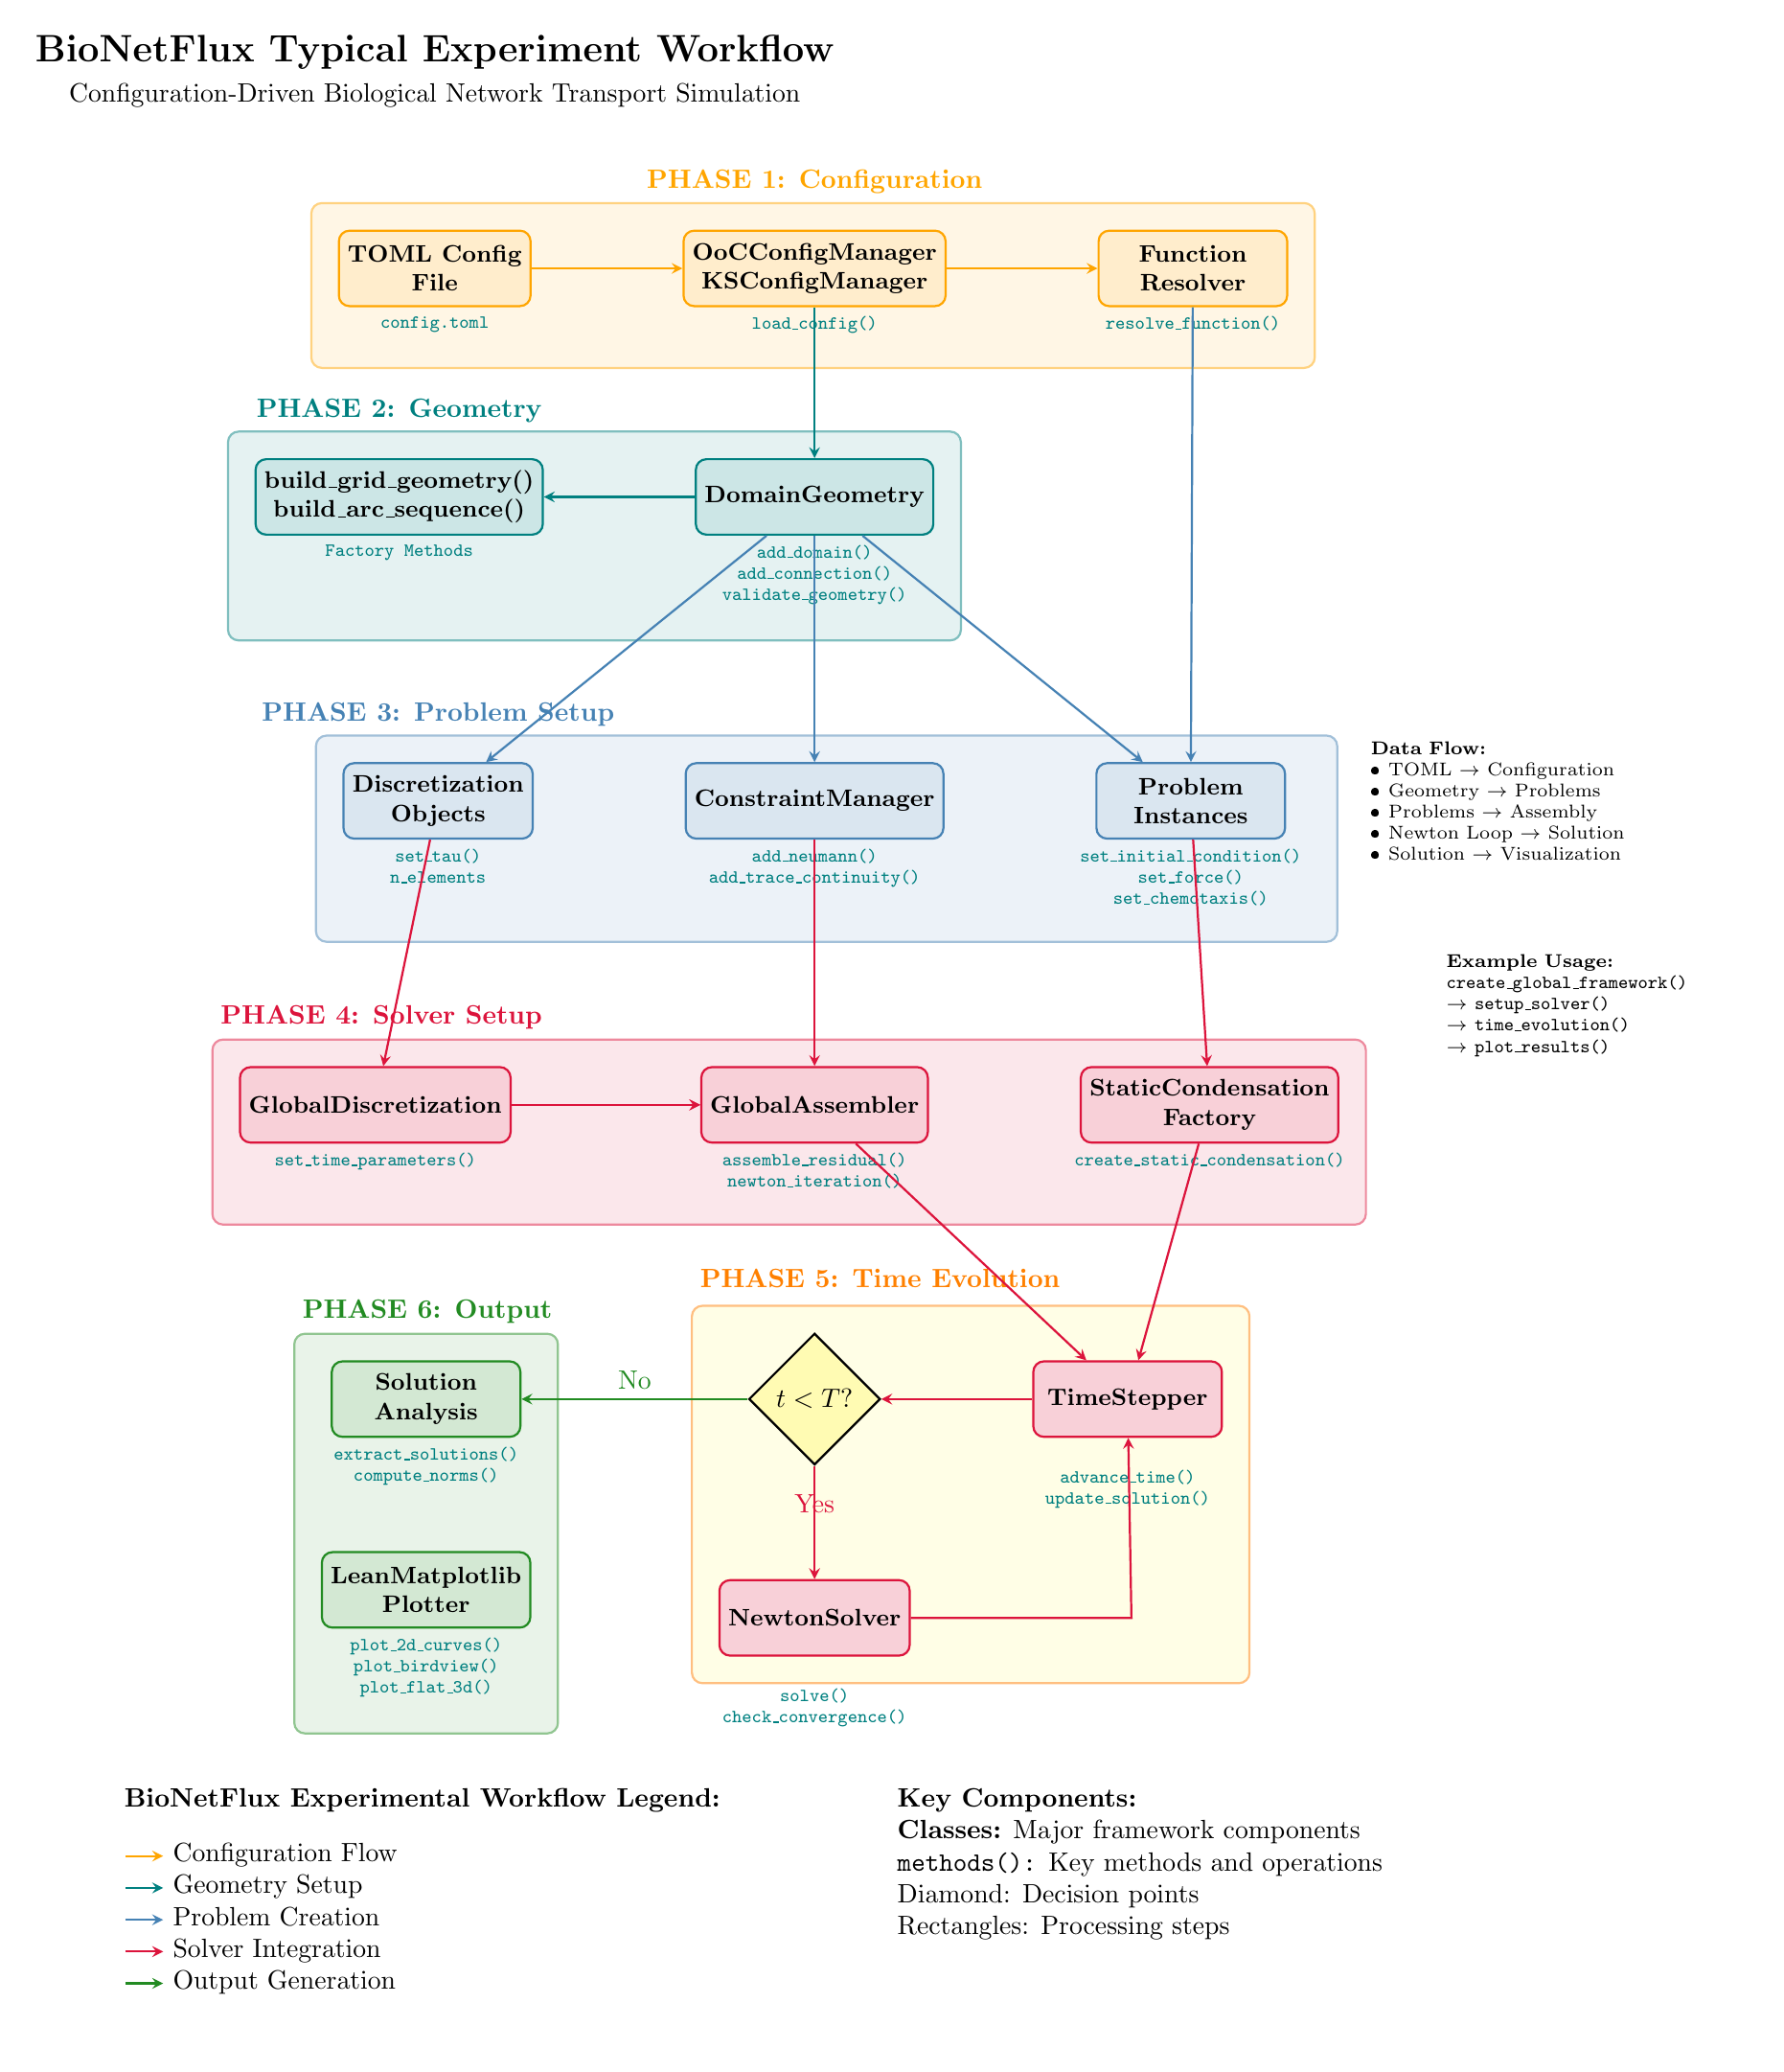
\begin{tikzpicture}[node distance=1.5cm and 2cm]

% ============================================================================
% PHASE 1: CONFIGURATION AND SETUP
% ============================================================================

% Configuration Phase
\node[configbox, classtext] (toml) {TOML Config\\File};
\node[configbox, right=of toml, classtext] (configmgr) {OoCConfigManager\\KSConfigManager};
\node[configbox, right=of configmgr, classtext] (resolver) {Function\\Resolver};

% Configuration methods
\node[methodtext, below=0.0cm of toml] (captiond) {\texttt{config.toml}};
\node[methodtext, below=0.0cm of configmgr] {\texttt{load\_config()}};
\node[methodtext, below=0.0cm of resolver] (captionf) {\texttt{resolve\_function()}};

% ============================================================================
% PHASE 2: GEOMETRY CREATION
% ============================================================================

% Geometry Phase
\node[geometrybox, below=2cm of configmgr, classtext] (geometry)  {DomainGeometry};
\node[geometrybox, left=of geometry, classtext] (factory) {build\_grid\_geometry()\\build\_arc\_sequence()};

% Geometry methods
\node[methodtext, below=0.0cm of geometry] (captione) {\texttt{add\_domain()}\\%
                                           \texttt{add\_connection()}\\%
                                           \texttt{validate\_geometry()}};
\node[methodtext, below=0.0cm of factory] {\texttt{Factory Methods}};

% ============================================================================
% PHASE 3: PROBLEM CREATION
% ============================================================================

% Problem Creation Phase
\node[problembox, below=3cm of geometry, classtext] (constraints) {ConstraintManager};
\node[problembox, right=of constraints, classtext] (problems) {Problem\\Instances};
\node[problembox, left=of constraints, classtext] (discretization) {Discretization\\Objects};


% Problem methods
\node[methodtext, below=0.0cm of problems] (captiona) {\texttt{set\_initial\_condition()}\\%
                                           \texttt{set\_force()}\\%
                                           \texttt{set\_chemotaxis()}};
\node[methodtext, below=0.0cm of discretization] (captionb) {\texttt{set\_tau()}\\%
                                                  \texttt{n\_elements}};
\node[methodtext, below=0.0cm of constraints] (captionc) {\texttt{add\_neumann()}\\%
                                              \texttt{add\_trace\_continuity()}};

% ============================================================================
% PHASE 4: SOLVER SETUP
% ============================================================================

% Solver Phase
\node[solverbox, below=3cm of constraints, classtext] (assembler) {GlobalAssembler};
\node[solverbox, left=2.5cm of assembler, classtext] (global_disc) {GlobalDiscretization};
\node[solverbox, right=of assembler, classtext] (static_cond) {StaticCondensation\\Factory};


% Solver methods
\node[methodtext, below=0.0cm of global_disc] {\texttt{set\_time\_parameters()}};
\node[methodtext, below=0.0cm of static_cond] {\texttt{create\_static\_condensation()}};
\node[methodtext, below=0.0cm of assembler] (captiong) {\texttt{assemble\_residual()}\\%
                                            \texttt{newton\_iteration()}};

% ============================================================================
% PHASE 5: TIME EVOLUTION
% ============================================================================

% Time Evolution Decision
\node[decision, below=2.5cm of assembler] (time_check) {$t < T$?};

% Newton Solver
\node[solverbox, right=2cm of time_check, classtext] (timestepper) {TimeStepper};
\node[methodtext, below=0.3cm of timestepper] (captioni) {\texttt{advance\_time()}\\%
	\texttt{update\_solution()}};



% Time Stepper
\node[solverbox, below=1.5cm of time_check, classtext] (newton) {NewtonSolver};
\node[methodtext, below=0.3cm of newton] {\texttt{solve()}\\%
	\texttt{check\_convergence()}};

% ============================================================================
% PHASE 6: OUTPUT AND VISUALIZATION
% ============================================================================

% Output Phase
\node[outputbox, left=3cm of time_check, classtext] (analysis) {Solution\\Analysis};
\node[outputbox, below=1.5cm of analysis, classtext] 
(plotter) {LeanMatplotlib\\Plotter};

% Output methods
\node[methodtext, below=0.0cm of plotter] (captionh) {\texttt{plot\_2d\_curves()}\\%
                                          \texttt{plot\_birdview()}\\%
                                          \texttt{plot\_flat\_3d()}};
\node[methodtext, below=0.0cm of analysis]  {\texttt{extract\_solutions()}\\%
                                           \texttt{compute\_norms()}};

% ============================================================================
% CONNECTIONS AND ARROWS
% ============================================================================

% Phase 1 connections
\draw[configarrow] (toml) -- (configmgr);
\draw[configarrow] (configmgr) -- (resolver);

% Phase 2 connections
\draw[geometryarrow] (configmgr) -- (geometry);
\draw[geometryarrow] (geometry) -- (factory);

% Phase 3 connections
\draw[problemarrow] (geometry) -- (problems);
\draw[problemarrow] (geometry) -- (discretization);
\draw[problemarrow] (geometry) -- (constraints);
\draw[problemarrow] (resolver) -- (problems);

% Phase 4 connections
\draw[solverarrow] (discretization) -- (global_disc);
\draw[solverarrow] (problems) -- (static_cond);
\draw[solverarrow] (constraints) -- (assembler);
\draw[solverarrow] (global_disc) -- (assembler);
\draw[solverarrow] (global_disc) -- (assembler);


% Phase 5 connections - Time evolution loop
\draw[solverarrow] (static_cond) -- (timestepper);
\draw[solverarrow] (assembler) -- (timestepper);
\draw[solverarrow] (timestepper) -- (time_check);

\draw[solverarrow] (time_check) -- node[above] {Yes} (newton);
\draw[solverarrow] (newton) -- ++(4.2,0) -- (timestepper);

% Phase 6 connections - Output
\draw[outputarrow] (time_check) -- node[above] {No} (analysis);

% ============================================================================
% BACKGROUND GROUPING
% ============================================================================

% Background rectangles for phases
\begin{scope}[on background layer]
    % Configuration Phase
    \node[fit=(toml)(configmgr)(resolver)(captiond), fill=configcolor!10, rounded corners, 
          draw=configcolor!50, thick, inner sep=10pt] {};
    \node[above=10pt of configmgr, configcolor, font=\bfseries] {PHASE 1: Configuration};
    
    % Geometry Phase  
    \node[fit=(geometry)(factory)(captione), fill=geometrycolor!10, rounded corners,
          draw=geometrycolor!50, thick, inner sep=10pt] {};
    \node[above=10pt of factory, geometrycolor, font=\bfseries] {PHASE 2: Geometry};
    
    % Problem Phase
    \node[fit=(problems)(discretization)(constraints)(captiona), fill=problemcolor!10, rounded corners,
          draw=problemcolor!50, thick, inner sep=10pt] {};
    \node[above=10pt of discretization, problemcolor, font=\bfseries] {PHASE 3: Problem Setup};
    
    % Solver Phase
    \node[fit=(global_disc)(static_cond)(assembler)(captiong), fill=solvercolor!10, rounded corners,
          draw=solvercolor!50, thick, inner sep=10pt] (boxsolver) {};
    \node[above=0cm of static_cond, solvercolor, font=\bfseries, anchor=south west] at (boxsolver.north west) {PHASE 4: Solver Setup};
    
    % Time Evolution Phase
    \node[fit=(time_check)(newton)(timestepper)(captioni), fill=yellow!10, rounded corners,
          draw=orange!50, thick, inner sep=10pt] (boxevolution) {};
    \node[above=0.1cm of time_check, orange, font=\bfseries, anchor=south west] at (boxevolution.north west)  {PHASE 5: Time Evolution};
    
    % Output Phase
    \node[fit=(plotter)(analysis)(captionh), fill=outputcolor!10, rounded corners,
          draw=outputcolor!50, thick, inner sep=10pt] (boxoutput) {};
    \node[above=0cm of analysis, outputcolor, font=\bfseries, anchor=south west] at (boxoutput.north west) {PHASE 6: Output};
\end{scope}

% ============================================================================
% LEGEND AND ANNOTATIONS
% ============================================================================

% Legend
\node[below=2cm of plotter] (legend) {
    \begin{minipage}{8cm}
        \textbf{BioNetFlux Experimental Workflow Legend:}\\[0.3cm]
        \tikz[baseline=-0.5ex] \draw[configarrow] (0,0) -- (0.5,0); Configuration Flow\\
        \tikz[baseline=-0.5ex] \draw[geometryarrow] (0,0) -- (0.5,0); Geometry Setup\\
        \tikz[baseline=-0.5ex] \draw[problemarrow] (0,0) -- (0.5,0); Problem Creation\\
        \tikz[baseline=-0.5ex] \draw[solverarrow] (0,0) -- (0.5,0); Solver Integration\\
        \tikz[baseline=-0.5ex] \draw[outputarrow] (0,0) -- (0.5,0); Output Generation\\[0.2cm]
    \end{minipage}
};

\node [right=2cm of legend, anchor=north west]  at (legend.north east) {
	\begin{minipage}{8cm}
		\textbf{Key Components:}\\
		\textbf{Classes:} Major framework components\\
		\texttt{methods():} Key methods and operations\\
		Diamond: Decision points\\
		Rectangles: Processing steps
	\end{minipage}
};
% Title and description
\node[above=2cm of toml, font=\Large\bfseries] {BioNetFlux Typical Experiment Workflow};
\node[above=1.5cm of toml, font=\normalsize] {Configuration-Driven Biological Network Transport Simulation};

% Data flow annotations
\node[right=1cm of problems, font=\scriptsize, text width=5cm, align=left] (dataflow) {
    \textbf{Data Flow:}\\
    • TOML $\rightarrow$ Configuration\\
    • Geometry $\rightarrow$ Problems\\  
    • Problems $\rightarrow$ Assembly\\
    • Newton Loop $\rightarrow$ Solution\\
    • Solution $\rightarrow$ Visualization
};

% Example workflow annotation
\node[below=1cm of dataflow, font=\scriptsize, text width=3cm, align=left] {
    \textbf{Example Usage:}\\
    \texttt{create\_global\_framework()}\\
    \texttt{$\rightarrow$ setup\_solver()}\\
    \texttt{$\rightarrow$ time\_evolution()}\\
    \texttt{$\rightarrow$ plot\_results()}
};

\end{tikzpicture}
\end{document}
